\hypertarget{nacionalismo-programuxe1tico}{%
\section{1830--1860: Nacionalismo
programático}\label{nacionalismo-programuxe1tico}}

\hypertarget{a-cidade-brasileira-do-suxe9culo-xix-e-a-construuxe7uxe3o-de-discursos-nacionais}{%
\subsection{A cidade brasileira do século XIX e a construção de
discursos
nacionais}\label{a-cidade-brasileira-do-suxe9culo-xix-e-a-construuxe7uxe3o-de-discursos-nacionais}}

A não centralidade do fato urbano na construção de discursos formativos
da nacionalidade brasileira, ao longo do século XIX, é evidenciada,
acima de tudo, na abstração indianista da literatura nacional. Como
lembra Zilá Bernd, a imagem do ``autóctone como antepassado mítico''
está atrelada a uma celebração sacralizada da natureza intocada ---
posto que o índio é parte dela, ao contrário do engenhoso português
\autocite[p.~37--38]{bernd:1992literatura}. Invisível desde o Rio de
Janeiro, cujos círculos literários são os produtores privilegiados dos
discursos sobre a nacionalidade, e combatida por missionários e
militares nas fronteiras demográficas do País, a espacialidade indígena
permanece ausente enquanto o índio idealizado faz furor na literatura da
segunda metade do século.

A mitológica harmonia do Romantismo entre português e indígena é
transposta para o Naturalismo do final do século, escancarando-se ao
mesmo tempo a exclusão do componente negro na formação étnica e cultural
brasileira, relegado por Euclides da Cunha a estrato racial e cultural
inferior ao do sertanejo mestiço de branco e índio
\autocite[p.~44]{bernd:1992literatura}, assim como reafirmando a
exclusividade luso-brasileira na produção do território.

De fato, o ordenamento jurídico construído ao longo do século XIX, em
especial pela Lei de Terras, não apenas reafirma a estratificação social
e racial na estrutura fundiária do País, como também restringe a
possível contribuição do imigrante ao processo de urbanização e ocupação
do território, colocando-a sempre sob a égide do Estado e dos grandes
proprietários já estabelecidos \autocite[p.~198]{depaula:2011processo}.

Se os textos críticos ou históricos na primeira metade do século XIX dão
pouco ou nenhum lugar à cidade e à urbanização, as representações
visuais do mesmo período compõem um acervo muito mais informativo. Desde
o período vice-real, afirma-se uma cultura visual secular que dá ao
primeiro discípulo brasileiro de Debret, Manuel de Araújo Porto Alegre
(1806--1879) ensejo para ver aí o primeiro ``impulso do espírito
nacional'' nas artes \autocite[p.~50]{magalhaes:1834resume}. Neste
contexto, destaca-se um \emph{corpus} imagético desconhecido ou
desconsiderado por Araújo Porto Alegre: a encomenda feita pelo Vice-rei
D. Luís de Vasconcelos e Sousa, conde de Figueiró, ao pintor e arquiteto
Leandro Joaquim (1738--1798), de uma série de vistas da cidade do Rio de
Janeiro destinadas a adornar o Passeio Público do Mestre Valentim,
completada em 1790 (Figura \ref{fig:joaquim}).

\begin{figure}
\hypertarget{fig:joaquim}{%
\centering
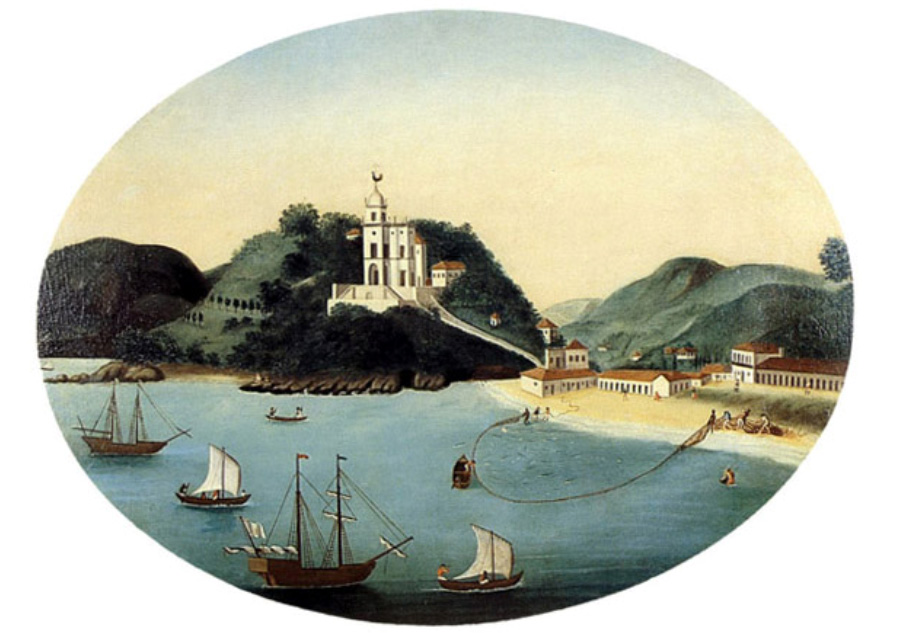
\includegraphics{figures/LeandroJoaquim-Gloria.jpg}
\caption{Leandro Joaquim (1738--1798). Igreja e Praia da Glória,
1790}\label{fig:joaquim}
}
\end{figure}

A série combina cenas oficiais de acontecimentos militares, ambientadas
no centro da cidade ou em seu porto, com representações, à primeira
vista anódinas, dos arredores da cidade. Não obstante a variedade de
cenas, a encomenda unitária sinaliza a intenção de formar uma imagem
global da sede administrativa do vice-reino para consumo interno. Assim,
distingue-se dos mapas e perfis urbanos produzidos para uso da Coroa
enquanto instrumentos de dominação, como os panoramas coetâneos de
Carlos Julião (1740--1811) e Luís dos Santos Vilhena (1744--1814),
aproximando-se do conjunto pictórico produzido pelos artistas franceses
a mando de D. João VI a partir de 1816. A chamada ``Missão artística
francesa'', vista desde Gonzaga Duque
\autocite[p.~257]{gonzagaduque:1995arte} até Bosi
\autocite[p.~228]{bosi:2011cultura} como um momento de ruptura com a
tradição colonial para inserção de um componente importado, insere-se,
pelo contrário, mais propriamente na continuidade do emergente cenário
de cultura urbana do Rio de Janeiro já promovido pelos vice-reis do que
se constituiria em inovação conceitual.

Nicolas-Antoine Taunay (1755--1830) e seu filho, Félix-Émile
(1795--1881), especializados em pintura de paisagem, produzem vasto
material iconográfico sobre o município da Corte, tanto em sua área
urbana quanto no entorno. O monumental panorama do Rio de Janeiro,
executado por Nicolas na França em 1824 com base em remessa de estudos
por Félix, tem lugar de honra nesse ciclo imagético cuja função evidente
é exaltar a dignidade da Capital do Reino e do Império perante a um
público europeu pouco afeito a reconhecer a legitimidade de um poder
ultramarino {[}\textcite{pereira:1994romantismo}; barata:1996alguns{]}.

Ressalta-se, por outro lado, a iconografia ``menor'' de Nicolas no Rio
de Janeiro, em particular as duas vistas do Outeiro da Glória. A
primeira composição, executada já em 1816, é visivelmente baseada na
mesma vista de Leandro Joaquim. Evidencia-se o reconhecimento, por parte
do recém-chegado francês, de uma cultura visual local, mais do que a
simples substituição da tradição colonial por um ``formalismo
indiferente à realidade brasileira''
\autocite[p.~49]{campofiorito:1983historia}. A segunda vista da Glória,
pintada em 1824, opera uma saborosa mescla do tema rococó do embarque
mítico, com reminiscências de Watteau, e de uma ênfase na paisagem
natural sobrepujando os elementos arquitetônicos (Figura
\ref{fig:nicolas}). Somente nesta última vista, executada pouco antes do
retorno de Nicolas à França, é que se percebe o início de um
distanciamento com respeito à pintura documental carioca do final do
século XVIII, substituída pelas referências mais diretas à arte europeia
recente.

\begin{figure}
\hypertarget{fig:nicolas}{%
\centering
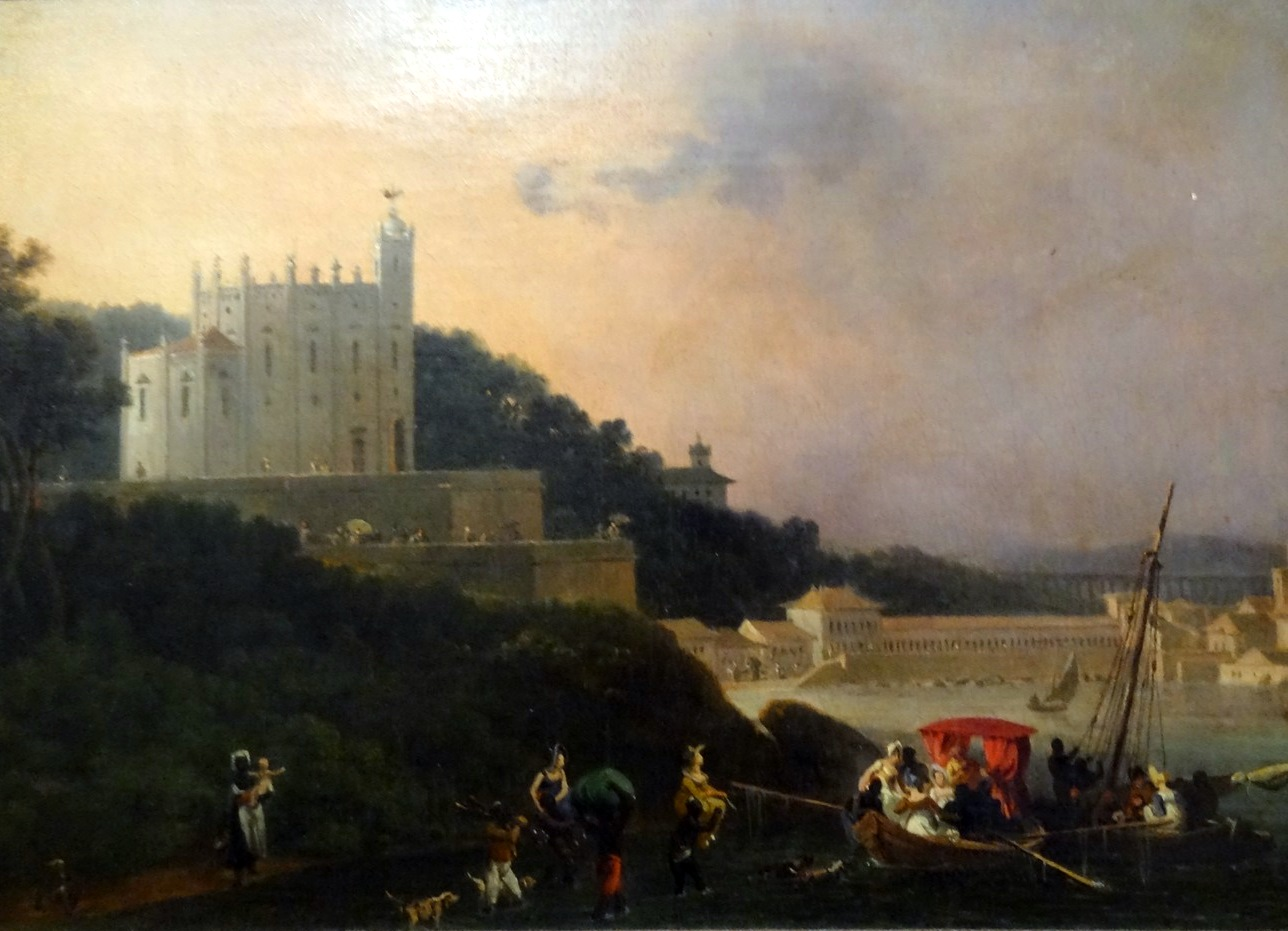
\includegraphics{figures/mar_rio_taunay_gloria_1824.jpeg}
\caption{Nicolas-Antoine Taunay (1755--1830). Glória,
1824}\label{fig:nicolas}
}
\end{figure}
